\documentclass[12pt,twoside]{article}
\renewcommand{\abstractname}{\vspace{-\baselineskip}}
\usepackage{hyperref}
\usepackage{setspace}
\usepackage{indentfirst}
\urlstyle{same}
\usepackage{geometry}
 \geometry{left=1.25in, right= 1.25in ,top=1.7in}
\setlength{\parindent}{.5in}
\renewcommand{\baselinestretch}{1.3}
\setlength{\parskip}{\baselineskip}
\usepackage{xcolor}
\usepackage{fancyhdr}
\usepackage{caption}
\captionsetup{font={normalsize,stretch=1}}
\renewcommand{\headrulewidth}{0pt}
\usepackage[labelfont=bf]{caption}
\captionsetup[figure]{labelfont={bf},name={Figure},labelsep=period}
\usepackage{natbib}
\setlength{\bibhang}{0.5in}
\bibliographystyle{apalike}
\usepackage{graphicx}
\usepackage{float}
%\usepackage{floatrow}
%  \floatsetup[table]{capposition=top}
\usepackage{booktabs}
\usepackage{tabularx}
\usepackage{titling}
\settowidth{\thanksmarkwidth}{*}
\setlength{\thanksmargin}{-\thanksmarkwidth}
\usepackage[hang,flushmargin]{footmisc}
\setlength{\skip\footins}{1.2pc plus 5pt minus 2pt}
\usepackage{titlesec}
\setlength{\droptitle}{-5em}
\setlength\thanksmarkwidth{.5em}
\setlength\thanksmargin{-\thanksmarkwidth}
\titleformat{\section}{\normalfont\bfseries\filcenter}{}{0pt}{}
\titleformat{\subsection}{\normalfont\bfseries\filcenter}{}{0pt}{\itshape}
\titleformat{\subsubsection}{\normalfont\bfseries\filcenter}{}{0pt}{\itshape}
\titlespacing*{\section}
  {0pt}{-.1\baselineskip}{-.1\baselineskip}  
\titlespacing*{\subsection}
   {0pt}{-.1\baselineskip}{-.1\baselineskip}  
\usepackage[T1]{fontenc}
\usepackage{fontspec}
  \fontspec{Times New Roman}
\date{}
\providecommand{\keywords}[1]
{
   \small	
  \textit{\hspace{-1em} Keywords: } #1
}
%\newfontfamily\headingfont[]{Times New Roman}
%Add Author names to headers and footers here:
\fancypagestyle{firstpage}{
  \fancyhf{}% clear all fields
  \fancyfoot[L]{ \footnotesize Copyright \copyright 2021 (Luehring et al.). Creative Commons Attribution-NonCommercial-NoDerivatives 4.0 International Public License. Available at: \url{http://journalqd.org}} 
  \lhead{ \footnotesize Journal of Quantitative Description: Digital Media 1(2021), 1–n} %Replace n with number of last page, including the Online Appendix.
\rhead{ \footnotesize 10.51685/jqd.2021.XXX}
}
\pagestyle{fancy}
\fancyhf{}
\fancyhead[LO]{ \footnotesize Journal of Quantitative Description: Digital Media 1(2021)}
\fancyhead[RO]{ \footnotesize Reviewing NewsGuard \thepage} %Select Short Title with fewer than 35 characters.
\fancyhead[LE]{ \footnotesize Luehring et al.} %(or Author1 et al.)
\fancyhead[RE]{ \footnotesize Journal of Quantitative Description: Digital Media 1(2021) \thepage}

%Article Title goes here
\title{ \normalsize \textbf{} \vspace{-1.5em}Reviewing domain-based approaches to track untrustworthy domains: How reliable is the NewsGuard database?} 
%Author names and affiliations go here in the single \author{} , put authors' contact information in \thanks{}. Use extra spacing: \vspace{1em} to separate authors (unless the authors share the same affiliation.  
\author{\normalsize Luehring, Jula \\ \normalsize University of Vienna & Complexity Science Hub, Vienna, Austria 
\vspace{1em} \\ \normalsize Lazzaroni, Ruggero Marino \\ \normalsize Lasser, Jana \\ \normalsize Institution, Country \thanks{\hspace{-1em} Author 1: jula.luehring@univie.ac.at} \thanks{\hspace{-1em} Author 2: author2's email address} \thanks{\hspace{-1em} Date submitted: XXXX-XX-XX}} 

\renewcommand\footnotemark{}
\begin{document}
\maketitle
\thispagestyle{firstpage}
\vspace{-8em}
\begin{abstract}
  \noindent \textbf{Abstract}
On social media, misinformation is widely visible \citep{lazerScienceFakeNews2018} and embedded in growing partisan sorting and intergroup conflict~\citep{gonzalez-bailonAsymmetricIdeologicalSegregation2023a}. To study these dynamics on digital platforms, it is imperative for computational social scientists to have access to reliable and valid tools that enable them to identify misinformation. A prominent way to track misinformation is to use a list of domains. The organization NewsGuard offers the most comprehensive database of domain trustworthiness ratings. Despite increasing popularity~\citep[for example,][]{robertsonUsersChooseEngage2023a,lasserSocialMediaSharing2022a}, the database was created as a tool for brand security rather than research, which is why access is not public and expensive. 
\end{abstract}
\keywords{\textit{misinformation, NewsGuard, social media} \vspace{8ex}}

\section{Introduction}
%The reach of misinformation on the general population has been debated (Watts et al., 2021), with only a small number of people engaging with misinformation online (Allen et al., 2020; Grinberg et al., 2019). Yet, when judging the consequences of the problem at the scale of the information ecosystem, misinformation seems to feed into growing partisan sorting and intergroup animosity (González-Bailón et al., 2023; Robertson et al., 2023). Misinformation is widely visible on social media and in the mainstream media (Tsfati et al., 2020), because it exploits the dynamics at play by fueling intergroup conflict and negative emotions. Consequently, it is imperative to understand the spread of misinformation and its interactions with digital media. In order to do so, computational social scientists need to have access to reliable and valid data. By reviewing strategies to research misinformation online, and assessing the reliability of source-based approaches in particular, we outline potential drawbacks and pitfalls for digital media research and offer recommendations for the application of the NewsGuard database in different contexts.


The spread of misinformation has been studied extensively by scholars from various scientific disciplines, therefore, relying on diverse conceptualizations. Definitions of misinformation seem to largely depend on the respective methodological choices, resulting in imprecise or inconclusive findings. To study the diffusion or discussion of misinformation on social media, computational researchers commonly use stories that were factchecked by experts, or follow blacklisted domains. The choice between story and source-based approaches hinges on the primary research objective. When operating at the level of the story, we capture misinformation with high precision, but the selection of stories can be narrow and is likely biased. Conversely, with a source-based strategy, we can cover a wider variety of sources and stories, and hence, the data may be less biased. However, this approach runs the risk of overgeneralizing across stories and source ratings may be especially sensitive to time and context. Therefore, we review different approaches to measuring misinformation online in terms of reliability, validity and feasibility and then focus on one perspective in particular that has recently gained popularity: domain-based approaches.



%In the United States, one of the most prominent lists used for assessing misinformation is curated by the organization \href{https://www.newsguardtech.com/ratings/rating-process-criteria/}{NewsGuard}. NewsGuard's analysts assign ratings based on nine distinct criteria and regularly update these assessments. The list has been increasingly used and research based in top-tiert journals (Robertson et al., 2023). However, there are several challenges associated with this list: First, the domain ratings were initially created as a tool for brand security rather than a research instrument, which is why the list is propriatory and access as well as publication of the data is restricted. Second, the coverage of the list has so far only been validated for research purposed for the U.S. context (Lin et al., 2023), but it is crucial to assess the usefulness of this list for research beyond the English-speaking world. Third, the list is updated in unknown intervals, which is why it is important to understand the update process and its implications for research. Fourth, the list is not exhaustive, which is why it is important to understand the selection process and its implications for research. Fifth, the list is not free of errors and missing data points, which is why it is important to understand their implications for research.

%Consequently, we propose to provide a comprehensive description of this database over time (monthly granularity) and across countries provided by NewsGuard. We believe that is is essential to address the following aspects of the database: the distribution, construction, weighting and update process of the ratings, the selection and removal of sources, and the completeness and reliability of other information provided in the database, e.g., political orientation.

%In addition, we reproduce published research relying on the NewsGuard list with different versions of the list to assess the degree to which results depend on a specific version of the list.

Therefore, we introduce our research question:
\begin{quotation}
  How reliable is the NewsGuard database of domain trustworthiness ratings
  over time and language contexts?
   \end{quotation}

More precisely, we describe the content of the NewsGuard database over time and across countries, focusing on three questions:
\begin{itemize}
    \item \textbf{How volatile are trustworthiness ratings, e.g., how often do ratings change or domains vanish?} This is important to estimate whether using an older database will distort results.
    \item \textbf{How reliable and complete is the provided information, particularly for non-US countries?} A recent study has shown high agreement of NewsGuard with other expert-rated lists in the U.S. context~\citep{linHighLevelCorrespondence2023}, but an assessment for other countries is missing. 
    \item \textbf{How can other information be used for misinformation research?} For each domain, NewsGuard rates journalistic quality criteria, topics, political slants, and labels AI-generated content. This information might shed light on aspects of misinformation beyond binary true/false labels.
\end{itemize}
By describing the database, we outline potential pitfalls and recommendations for digital media research. We also want to empower misinformation researchers to make informed decisions about whether the substantial expense associated with acquiring access to NewsGuard is necessary for their research. 
\subsection*{NewsGuard}
NewsGuard rates outlets based on web traffic data, claiming that they have reviewed domains accounting for 95\% of online engagement. The organization sometimes adds outlets they deem influential or that changed domains. NewsGuard saves hourly snapshots of the database, allowing us to track changes going back to March 2019, when the organization started operating. 
Notably, NewsGuard is not a blacklist. In fact, close to 60\% of domains have an overall rating of over 60 and are therefore considered ``trustworthy''(see Fig.~\ref{fig:fig1}) for the distribution of trustworthiness scores. 
\begin{figure}[!ht]
    \centering
    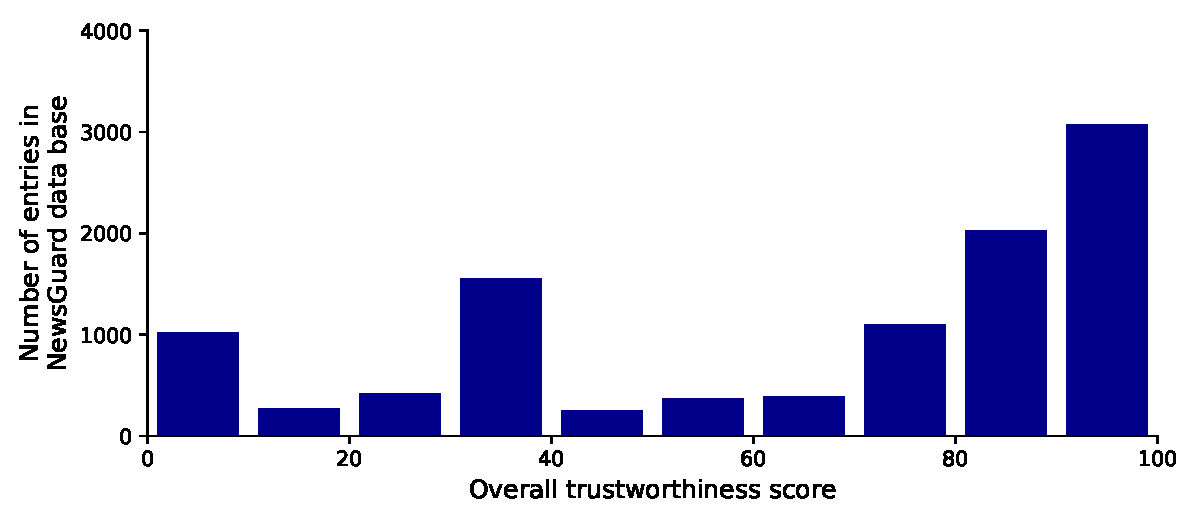
\includegraphics[width=\textwidth]{NewsGuard_histogram.pdf}
    \caption{Distribution of domain trustworthiness contained in the NewsGuard database as of September 20, 2023.}
    \label{fig:fig1}
\end{figure}
NewsGuard experts regularly assess the trustworthiness of news outlets. As of September 20, 2023, the database contains 10,993 trustworthiness assessments, including:
\begin{itemize}
    \item Domain and trustworthiness rating (between 0 and 100).
    \item Binary labels (yes/no) for nine journalistic quality criteria constituting the trustworthiness rating. Criteria are, for example, ``Regularly corrects or clarifies errors'' (12.5 points) or ``Gathers and presents information responsibly'' (18 points)\footnote{See \href{https://www.newsguardtech.com/ratings/rating-process-criteria/}{https://www.newsguardtech.com/ratings/rating-process-criteria/} for a full list.}
    \item Language and country associated with the domain,  covering nine countries as well as a ```global``` label, and five languages (English, Italian, French, German, Spanish). Most assessments are from the US (66\%), followed by global domains (12\%), Great Britain (5\%), Italy (5\%), Canada (4\%), France (4\%) and Germany (3\%).
    \item Topics covered (e.g., ``local news'', ``political news'', ``health information'') and political orientation (left/right).
    \item A flag indicating whether the outlet frequently posts AI-generated content.
\end{itemize}

\section{Results}
\subsection{Coverage}
\subsubsection{Replicability}

\section{Discussion}

\section{Methods}

\section{Acknowledgments}
Acknowledgements/ Author's disclosure/ funding statement.

\bibliography{newsguard-review.bib}

\appendix
\section{Online Appendix}
Appendix goes here.
\end{document}

\bibliography{newsguard-review.bib}
\end{document}

%%MISC TEXT
%How and when are ratings updated? How important is it to use up-to-date ratings? 
%How many sources are added and dropped? Do I need to use multiple versions of the database, or is it enough to use one/the latest snapshots? How do the results of our research projects change with different versions of NewsGuard? What is the coverage of countries and languages? 
%Alternative information: Political orientation? How do different rating criteria contribute to the overall ratings?  

%In practice, however, it is challenging to draw a line on truth; and it is even more challenging to identify the exact intention behind a misleading tweet (REF). Concerning the latter dimension (the intention), scholars distinguish disinformation and fake news, typically pushing an economic or political agenda, from other types of false information with no particular or unclear purpose (Wardle \& Derakhshan, 2017). In observational research concentrating on perceptive aspects instead of the exact intention, researchers often apply misinformation as an umbrella term (Weeks \& Gil de Zúñiga, 2021). We follow this rationale that shifts the focus to the outcome rather than the production of misinformation and account for the second dimension (the facticity) by treating news reliability as a continuum.

%Underestimation of subtle types of misinformation: Few people are exposed to misinformation, but most people have partisan information diets. Here, falseness is a continuum, and misinformation is a means to an end. Therefore, the degree of falseness is central to capturing the problem scope and, especially for computational scientists, reviewing this phenomenon at the scale of the information ecosystem. 

%from LOI

%The spread of misinformation has been studied extensively by scholars from various scientific disciplines, therefore, relying on diverse conceptualizations. Definitions of misinformation seem to largely depend on the respective methodological choices, resulting in imprecise or inconclusive findings \citep{altayMisinformationMisinformationConceptual2023a}.
%The choice between story and source-based approaches hinges on the primary research objective. When operating at the level of the story, we capture misinformation with high precision, but the selection of stories can be narrow and is likely biased. Conversely, with a source-based strategy, we can cover a wider variety of sources and stories, and hence, the data may be less biased. However, this approach runs the risk of overgeneralizing across stories and source ratings may be especially sensitive to time and context. 

%For the U.S. context, the list has shown high agreement with other expert-rated lists \citep{linHighLevelCorrespondence2023}, but it is crucial to assess the usefulness for research beyond the English-speaking world. Moreover, the ratings were initially created as a tool for brand security rather than a research instrument, which is why access as well as publication of the data is restricted. %Second, ratings and sources are updated in unknown intervals, which is why it is important to understand the update process of the ratings as well as changes in source coverage. 
% Finally, it remains unclear how inconsistencies in source selection, reliability ratings and other categories rated by NewsGuard would affect the results of a study. Therefore, we propose to provide a comprehensive description of this database over time and across countries by addressing the following aspects of the database: 
% \begin{enumerate}[label= \alph*)]
% \item the distribution, construction, weighting and update process of the ratings,
% \item the selection and removal of sources, and 
% \item the completeness and reliability of other information provided in the database, e.g., political orientation.
% \end{enumerate}

% In addition, we reproduce published research relying on the NewsGuard list with different versions of the list to assess the degree to which results depend on a specific version of the list.

%Given that we have access to the entire NewsGuard database, we constructed a sample by merging all lists with monthly granularity, covering March 2019 until March 2023. Over four years, the dataset has grown from 2,622 to 10,993 sources, and now covers 9 countries (United States, Italy, Great Britain, France, Germany, Canada, Australia, Austria, New Zealand) and five different languages (English, Italian, French, German, Spanish). Yet, %the dataset is not balanced across countries and languages: 
%the majority of the sources (76\%) are in English and come from the United States. After analyzing global trends for the whole sample, we subset the non-U.S. data and compare across those countries.

%\section*{How does it pertain to digital media?}
%The reach of misinformation on the general population has been debated \citep{wattsMeasuringNewsIts2021b}, with only a small number of people engaging with misinformation online \citep{allenEvaluatingFakeNews2020,grinbergFakeNewsTwitter2019}. Yet, 
% When judging the consequences of misinformation at the scale of the information ecosystem \citep{allenEvaluatingFakeNews2020}, it feeds into a system shaped by growing partisan sorting and intergroup animosity \citep{gonzalez-bailonAsymmetricIdeologicalSegregation2023a, robertsonUsersChooseEngage2023a}. Misinformation is widely visible on social media \citep{lazerScienceFakeNews2018} and in the mainstream media \citep{tsfatiCausesConsequencesMainstream2020}, because it exploits the dynamics at play by fueling intergroup conflict and negative emotions. Consequently, to understand the spread of misinformation on digital platforms, it is imperative for computational social scientists to have access to reliable and valid data. By assessing the reliability of source-based approaches, we outline potential pitfalls for digital media research and offer recommendations for the application of the NewsGuard database in different countries.